\documentclass[journal,12pt,twocolumn]{IEEEtran}
%
\usepackage{setspace}
\usepackage{gensymb}
%\doublespacing
\singlespacing

%\usepackage{graphicx}
%\usepackage{amssymb}
%\usepackage{relsize}
\usepackage[cmex10]{amsmath}
%\usepackage{amsthm}
%\interdisplaylinepenalty=2500
%\savesymbol{iint}
%\usepackage{txfonts}
%\restoresymbol{TXF}{iint}
%\usepackage{wasysym}
\usepackage{amsthm}
%\usepackage{iithtlc}
\usepackage{mathrsfs}
\usepackage{txfonts}
\usepackage{stfloats}
\usepackage{bm}
\usepackage{cite}
\usepackage{cases}
\usepackage{subfig}
%\usepackage{xtab}
\usepackage{longtable}
\usepackage{multirow}
%\usepackage{algorithm}
%\usepackage{algpseudocode}
\usepackage{enumitem}
\usepackage{mathtools}
\usepackage{steinmetz}
\usepackage{tikz}
\usepackage{circuitikz}
\usepackage{verbatim}
\usepackage{tfrupee}
\usepackage[breaklinks=true]{hyperref}
%\usepackage{stmaryrd}
\usepackage{tkz-euclide} % loads  TikZ and tkz-base
%\usetkzobj{all}
\usetikzlibrary{calc,math}
\usepackage{listings}
    \usepackage{color}                                            %%
    \usepackage{array}                                            %%
    \usepackage{longtable}                                        %%
    \usepackage{calc}                                             %%
    \usepackage{multirow}                                         %%
    \usepackage{hhline}                                           %%
    \usepackage{ifthen}                                           %%
  %optionally (for landscape tables embedded in another document): %%
    \usepackage{lscape}     
\usepackage{multicol}
\usepackage{chngcntr}
%\usepackage{enumerate}

%\usepackage{wasysym}
%\newcounter{MYtempeqncnt}
\DeclareMathOperator*{\Res}{Res}
%\renewcommand{\baselinestretch}{2}
\renewcommand\thesection{\arabic{section}}
\renewcommand\thesubsection{\thesection.\arabic{subsection}}
\renewcommand\thesubsubsection{\thesubsection.\arabic{subsubsection}}

\renewcommand\thesectiondis{\arabic{section}}
\renewcommand\thesubsectiondis{\thesectiondis.\arabic{subsection}}
\renewcommand\thesubsubsectiondis{\thesubsectiondis.\arabic{subsubsection}}

% correct bad hyphenation here
\hyphenation{op-tical net-works semi-conduc-tor}
\def\inputGnumericTable{}                                 %%

\lstset{
%language=C,
frame=single, 
breaklines=true,
columns=fullflexible
}
%\lstset{
%language=tex,
%frame=single, 
%breaklines=true
%}


\begin{document}
%


\newtheorem{theorem}{Theorem}[section]
\newtheorem{problem}{Problem}
\newtheorem{proposition}{Proposition}[section]
\newtheorem{lemma}{Lemma}[section]
\newtheorem{corollary}[theorem]{Corollary}
\newtheorem{example}{Example}[section]
\newtheorem{definition}[problem]{Definition}
%\newtheorem{thm}{Theorem}[section] 
%\newtheorem{defn}[thm]{Definition}
%\newtheorem{algorithm}{Algorithm}[section]
%\newtheorem{cor}{Corollary}
\newcommand{\BEQA}{\begin{eqnarray}}
\newcommand{\EEQA}{\end{eqnarray}}
\newcommand{\define}{\stackrel{\triangle}{=}}

\bibliographystyle{IEEEtran}
%\bibliographystyle{ieeetr}


\providecommand{\mbf}{\mathbf}
\providecommand{\pr}[1]{\ensuremath{\Pr\left(#1\right)}}
\providecommand{\qfunc}[1]{\ensuremath{Q\left(#1\right)}}
\providecommand{\sbrak}[1]{\ensuremath{{}\left[#1\right]}}
\providecommand{\lsbrak}[1]{\ensuremath{{}\left[#1\right.}}
\providecommand{\rsbrak}[1]{\ensuremath{{}\left.#1\right]}}
\providecommand{\brak}[1]{\ensuremath{\left(#1\right)}}
\providecommand{\lbrak}[1]{\ensuremath{\left(#1\right.}}
\providecommand{\rbrak}[1]{\ensuremath{\left.#1\right)}}
\providecommand{\cbrak}[1]{\ensuremath{\left\{#1\right\}}}
\providecommand{\lcbrak}[1]{\ensuremath{\left\{#1\right.}}
\providecommand{\rcbrak}[1]{\ensuremath{\left.#1\right\}}}
\theoremstyle{remark}
\newtheorem{rem}{Remark}
\newcommand{\sgn}{\mathop{\mathrm{sgn}}}
\providecommand{\abs}[1]{\left\vert#1\right\vert}
\providecommand{\res}[1]{\Res\displaylimits_{#1}} 
\providecommand{\norm}[1]{\left\lVert#1\right\rVert}
%\providecommand{\norm}[1]{\lVert#1\rVert}
\providecommand{\mtx}[1]{\mathbf{#1}}
\providecommand{\mean}[1]{E\left[ #1 \right]}
\providecommand{\fourier}{\overset{\mathcal{F}}{ \rightleftharpoons}}
%\providecommand{\hilbert}{\overset{\mathcal{H}}{ \rightleftharpoons}}
\providecommand{\system}{\overset{\mathcal{H}}{ \longleftrightarrow}}
	%\newcommand{\solution}[2]{\textbf{Solution:}{#1}}
\newcommand{\solution}{\noindent \textbf{Solution: }}
\newcommand{\cosec}{\,\text{cosec}\,}
\providecommand{\dec}[2]{\ensuremath{\overset{#1}{\underset{#2}{\gtrless}}}}
\newcommand{\myvec}[1]{\ensuremath{\begin{pmatrix}#1\end{pmatrix}}}
\newcommand{\mydet}[1]{\ensuremath{\begin{vmatrix}#1\end{vmatrix}}}
%\numberwithin{equation}{section}
\numberwithin{equation}{subsection}
%\numberwithin{problem}{section}
%\numberwithin{definition}{section}
\makeatletter
\@addtoreset{figure}{problem}
\makeatother

\let\StandardTheFigure\thefigure
\let\vec\mathbf
%\renewcommand{\thefigure}{\theproblem.\arabic{figure}}
\renewcommand{\thefigure}{\theproblem}
%\setlist[enumerate,1]{before=\renewcommand\theequation{\theenumi.\arabic{equation}}
%\counterwithin{equation}{enumi}


%\renewcommand{\theequation}{\arabic{subsection}.\arabic{equation}}

\def\putbox#1#2#3{\makebox[0in][l]{\makebox[#1][l]{}\raisebox{\baselineskip}[0in][0in]{\raisebox{#2}[0in][0in]{#3}}}}
     \def\rightbox#1{\makebox[0in][r]{#1}}
     \def\centbox#1{\makebox[0in]{#1}}
     \def\topbox#1{\raisebox{-\baselineskip}[0in][0in]{#1}}
     \def\midbox#1{\raisebox{-0.5\baselineskip}[0in][0in]{#1}}

\vspace{3cm}


\title{Quiz 9}
\author{S Nithish}
% make the title area
\maketitle

\newpage

%\tableofcontents

\bigskip

\renewcommand{\thefigure}{\theenumi}
\renewcommand{\thetable}{\theenumi}
%\renewcommand{\theequation}{\theenumi}


\begin{abstract}
This document contains the solution of the question from NCERT 9th standard chapter 10 exercise 10.4 problem 4
\end{abstract}

%Download all python codes 
%
%\begin{lstlisting}
%svn co https://github.com/JayatiD93/trunk/My_solution_design/codes
%\end{lstlisting}

%Download all and latex-tikz codes from 
%
%\begin{lstlisting}
%svn co https://github.com/gadepall/school/trunk/ncert/geometry/figs
%\end{lstlisting}
%
\section{Exercise 10.4}
\begin{enumerate}
	\item If a line intersects two concentric circles with centre O at A,B,C and D, prove that AB=CD.

\begin{figure}[ht]
	\centering
	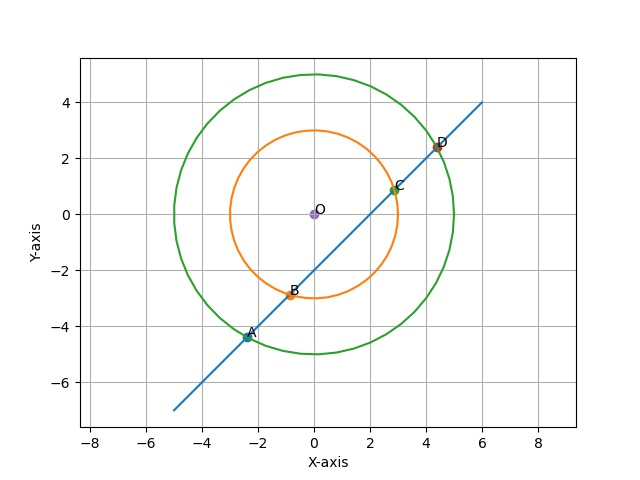
\includegraphics[width = \columnwidth]{figs/plot.jpg}
	\caption{Circle}
	\label{fig:1}
\end{figure}

Let the inner circle be of radius 3 and the outer circle be of radius 5. Then the equation of the two circles are,

		\begin{align}
			\norm{\vec{x}} &= 9\\
			\norm{\vec{x}} &= 25
		\end{align}

Let the equation of the line be,

		\begin{align}
			\vec{x} = \vec{h} +\mu \vec{m}\\
		\end{align}

The equation of the conic section is,

		\begin{align}
			\text{g}(\vec{x}) = \vec{x}^{\top}\vec{V}\vec{x} +2\vec{u}^{\top}\vec{x} + f=0
		\end{align}
Then the parameter $\mu$ for the points of intersection of the line with the conic is given by,
		\begin{align}
			\mu^2\vec{m}^{\top}\vec{V}\vec{m}+2\mu\vec{m}^{\top}\brak{\vec{V}\vec{h}+\vec{u}} +\text{g}(\vec{h}) = 0
		\end{align}

Two have 2 points of intersection the above quadratic equation must have positive discriminant.

		\begin{align}
			4\brak{\vec{m}^{\top}\brak{\vec{V}\vec{h}+\vec{u}}}^2-4\brak{\vec{m}^{\top}\vec{V}\vec{m}}\brak{\text{g}(\vec{h})}>0
		\end{align}

As the circles are concentric we can say that if the line intersects the inner circle at two points it will intersect the outter circle at two points.

		\begin{align}
			\vec{V} = \vec{I}, \text{ } \vec{u} = \vec{O}, \text{ } f = -9 
		\end{align}
The line we have considered is,

		\begin{align}
			\vec{x} &= \myvec{0\\-2}+\mu\myvec{1\\1}\\
			\vec{m} &= \myvec{1\\1}\\
			\vec{h} &= \myvec{0\\-2}\\
			\vec{m}^{\top}\vec{V}\vec{m} &= 2\\
			\vec{m}^{\top}\brak{\vec{V}\vec{h}+\vec{u}}&=-2\\
			g(\vec{h}) &= -5\\
			\implies 4\brak{\vec{m}^{\top}\brak{\vec{V}\vec{h}+\vec{u}}}^2&-4\brak{\vec{m}^{\top}\vec{V}\vec{m}}\brak{\text{g}(\vec{h})}\\
			&=4\brak{-2}^2-4\brak{2}\brak{-5}\\
			&=56>0
		\end{align}


The point of intersection of the line and the inner circle is,

		\begin{align}
			2\mu^2-4\mu-5=0\\
			\mu_b = \frac{4-\sqrt{56}}{4} = 1-\sqrt{\frac{7}{2}}\\
			\mu_c = \frac{4+\sqrt{56}}{4} = 1+\sqrt{\frac{7}{2}}
		\end{align}

		\begin{align}
			\vec{x} &= \myvec{0\\-2}+\lambda \myvec{1\\1}\\
			\vec{x} &= \myvec{\lambda \\ \lambda - 2}
		\end{align}

The point of intersection of the line and the outter circle is,

		\begin{align}
			\vec{V} = \vec{I}, \vec{u}=\vec{O},f=-25\\
			g(\vec{h}) = 4-25=-21\\
		\end{align}	
The remaining terms remains same as in the previous case.

		\begin{align}
			2\mu^2-4\mu-21=0\\
			\mu_a = \frac{4-\sqrt{184}}{4} = 1-\sqrt{\frac{23}{2}}\\
			\mu_d = \frac{4+\sqrt{184}}{4} = 1+\sqrt{\frac{23}{2}}\\
		\end{align}

Hence the points A,B,C and D are,
\begin{align}
	\vec{x_a} = \myvec{1-\sqrt{\frac{23}{2}}\\-1-\sqrt{\frac{23}{2}}}\\
	\vec{x_b} = \myvec{1-\sqrt{\frac{7}{2}}\\-1-\sqrt{\frac{7}{2}}}\\
	\vec{x_c} = \myvec{1+\sqrt{\frac{7}{2}}\\-1+\sqrt{\frac{7}{2}}}\\
	\vec{x_a} = \myvec{1+\sqrt{\frac{23}{2}}\\-1+\sqrt{\frac{23}{2}}}\\
\end{align}
The distance between points A and B is,

		\begin{align}
			AB = \norm{\vec{x_a}-\vec{x_b}} &= \norm{\myvec{\frac{\sqrt{7}-\sqrt{23}}{\sqrt{2}}\\\frac{\sqrt{7}-\sqrt{23}}{\sqrt{2}}}} = \sqrt{23}-\sqrt{7}\\
			CD = \norm{\vec{x_c}-\vec{x_d}} &= \norm{\myvec{\frac{\sqrt{7}-\sqrt{23}}{\sqrt{2}}\\\frac{\sqrt{7}-\sqrt{23}}{\sqrt{2}}}} = \sqrt{23}-\sqrt{7}\\
			\implies AB=CD
		\end{align}

\end{enumerate}

%\begin{enumerate}[label=\thesection.\arabic*.,ref=\thesection.\theenumi]
%\num then what are its direction cosines ?berwithin{equation}{enumi}
%\item Verification of the above problem using python code.\\
%%\solution The  following Python code generates Fig. \ref{fig:point_distance}
%%\begin{lstlisting}
%%codes/det_check.py
%%\end{lstlisting}
%
%\end{enumerate}

\end{document}

